\section{Testing and beyond}
\label{sec:conclusion:testing}

Despite the promising results obtained by \textit{Autofunk} in
Chapter \ref{sec:testing}, there is room for improvement. The
next section is focused on \textit{Autofunk}'s usability, \emph{i.e.}
how, we think, \textit{Autofunk} could be enhanced to be more
widely used. Furthermore, in this thesis, we only covered passive
testing of production systems, but it would be interesting to see
how active testing could be integrated with \textit{Autofunk}.
This is discussed in Section \ref{sec:conclusion:testing:active}.
Section \ref{sec:conclusion:testing:data} introduces our thoughts
on data mining, which are semi-related to the previous section on
active testing. Finally, Section
\ref{sec:conclusion:testing:valid} discusses our main assumption
used throughout this thesis, \emph{i.e.} we infer models of
systems that behave correctly, and what we could do to reject it.

%%%%%%%%%%%%%%%%%%%%%%%%%%%%%%%%%%%%%%%%%%%%%%%%%%%%%%%%%%%%%%%%

\subsection{Improving usability}

Our implementation of \textit{Autofunk} has primarily been built
to validate our work, but also to fill the gap between research
and industrial applicability, thanks to our partner Michelin. At
the time of writing, \emph{Autofunk} is a Java console
application with about 3,000 lines of code, and 119 unit tests
covering 90\% of the code.

Nevertheless, it is clear that this tool is still a prototype,
and not a production-ready tool. As pointed out in this thesis,
memory consumption remains an issue for example, because we load
all objects in memory in order to act on them. At the time of
writing, we partially fixed this problem by reducing
\emph{Autofunk}'s memory footprint with better object
representations in memory, but it is not future-proof.
With the rise of big data technologies and tools, it should be
possible to find a better solution to this issue. For instance,
\emph{Autofunk v3} includes \emph{Apache
Spark}\footnote{\url{https://spark.apache.org/}}, a framework for
large-scale data processing, which, among all, provides an
implementation of the k-means clustering algorithm.  Such a
framework is designed to handle large data sets. It should be
possible to make \emph{Autofunk} more efficient by adapting our
algorithms on-top of Apache Spark or any similar big data
framework, \emph{e.g.}, with a \emph{Map-Reduce} approach
\cite{dean2008mapreduce}. This is a programming model that allows
to process large data sets with distributed parallel algorithms.
Most of the algorithms presented in this thesis are already
executable in parallel, but not distributed yet. Nonetheless,
running \emph{Autofunk} on a computer cluster, \emph{i.e.} a set
of interconnected computers seen as a single logical unit, should
bring significant performance improvements, but it should also
refine the overall scalability.

By now, inference rules written with the Drools rule language,
which are at the heart of \emph{Autofunk}, have to be packaged
within the Java application. It would be better to allow the
configuration of such rules at runtime, \emph{e.g.}, using a
graphical user interface. This could also be helpful to write and
manage the different sets of inference rules, which is an issue
we already mentioned earlier in this thesis. An interface may
mitigate such a drawback, but writing such inference rules
remains a delicate task. That is why we would like to investigate
different approaches to avoid such a labor. As we are already
familiar with machine learning, we would like to pursue in this
path by proposing a machine learning technique that replaces some
of the inference rules. For instance, because the events in a
production system are text-based and readable, the inference
rules needed during the filtering step might be replaced by a
method inspired by the works on automated text categorization
\cite{Sebastiani:2002:MLA:505282.505283}. Yet, it is manifest
that the inference rules used to lift abstraction of the models
still have to be written, and cannot be easily replaced, because
they strongly depend on the business.

Another point that would be worth working on is the
\emph{visualization} of the inferred models and test results. At
the time of writing, \emph{Autofunk} is able to generate graphs
representing the generated models, but they are not really usable
in practice because of the size of the models. In most cases, the
models represent behaviors of a production system. The models fit a system's
physical layout in a factory. When a possibly fail trace is
raised, it would be nice to highlight the possibly faulty
behavior directly using the layout of the production system under
test. That way, an engineer would have all the information
required to quickly determine what caused such a behavior, and
state whether it is a bug or a false positive. We could relate
this idea to the research field on \emph{fault localization}
\cite{jones2002visualization,wong2010software}, except that we
would locate faults in a physical manner in a factory.

Finally, we would like to reduce the number of false positives
yield by our test engine as presented in
\crossref{sec:testing}{sec:testing:offline:impl-exp}. For the
record, false positives are behaviors that are considered
possibly faulty, even though they are correct, because such
behaviors are not part of the reference models. We already know
that inferring reference models from large sets of traces reduces
the number of false positives, but there might be other methods
to overcome this issue. For instance, we proposed a weaker
implementation relation that works well to avoid false positives
with similar behaviors that are (partially) known. Unfortunately,
this is not simply a problem of \emph{safe} (regression) test
selection \cite{orso2004scaling} because we cannot plainly reject
all new behaviors (as we could do in some more traditional
testing scenarios). A naive approach would be to teach the test
engine to recognize the new yet correct behaviors, but it seems
cumbersome. Instead, we believe that enabling active testing may
be more effective.

%%%%%%%%%%%%%%%%%%%%%%%%%%%%%%%%%%%%%%%%%%%%%%%%%%%%%%%%%%%%%%%%

\subsection{Performing active testing}
\label{sec:conclusion:testing:active}

Active testing, as defined in
\crossref{sec:related:testing}{sec:related:testing:active-passive},
works by stimulating a system under test. We chose not to take
this direction because stimulating a production system might
break it if one sends incorrect data. Indeed, as there are
physical devices behind software, it could lead to severe
damages.  Nonetheless, and according to our partner Michelin, it
should be possible to reproduce a production environment in a
simulation room, and thus to simulate a whole production system
without the physical devices (only the logical controllers). We
could then leverage our inferred models, which contain the data
collected from a real environment, to construct the test cases,
and execute them in an active testing approach.

The main benefit of active testing would be to avoid collecting
traces of the system under test for a long period, and directly
test this system instead. We believe that adding active testing
to \textit{Autofunk} would speed up the testing process
significantly, and it would also make its adoption easier as
active testing is more often known than passive testing in the
Industry.

A simplistic way to perform active testing would be to "replay"
\cite{thane2000using,Orso:2005:SCR:1082983.1083251} the data
previously "recorded", \emph{i.e.} the data available in the
inferred models. This is a path Michelin would like to explore.
Figure \ref{fig:autofunk_active} gives the insight of their use
case. A system under analysis $\mathit{Sua}$ in a production
environment is used to build a first set of models. A system
under test $\mathit{Sut}$, which is likely a different version of
the system under analysis, is set up in a simulation environment
(as already mentioned before).  Replaying the data from
$\mathit{Sua}$ in $\mathit{Sut}$ should produce new events that
would be used to infer models of $\mathit{Sut}$.  At this point,
it should be possible to reuse the passive testing technique
described in this thesis.  Nevertheless, the main unanswered
question is how to replay the data in a safe manner?  Such an
approach also implies that the initial conditions are exactly the
same between the system under analysis and the system under test.
This is yet another strong assumption we would prefer not to
make.

Instead, we would like to leverage our inferred models to extract
test data, for instance, by mining \emph{realistic domains} as
defined in \cite{Enderlin:2011:PSL:2075545.2075551}. Realistic
domains are data domains found in concrete implementations. A
data domain should come with a practical way to generate values
in it. This would be particularly useful to actively test a
system as it would ease the process of generating test data by
means of a sampler for instance, \emph{i.e.} a value generator.

Mining realistic domains for testing purpose is not the only use
case in which we believe. Indeed, our inferred models own a lot
of interesting information related to the behaviors of a
production system running in production, and it could be
interesting to apply data mining techniques on them.\\

\begin{figure}[h]
    \begin{center}
        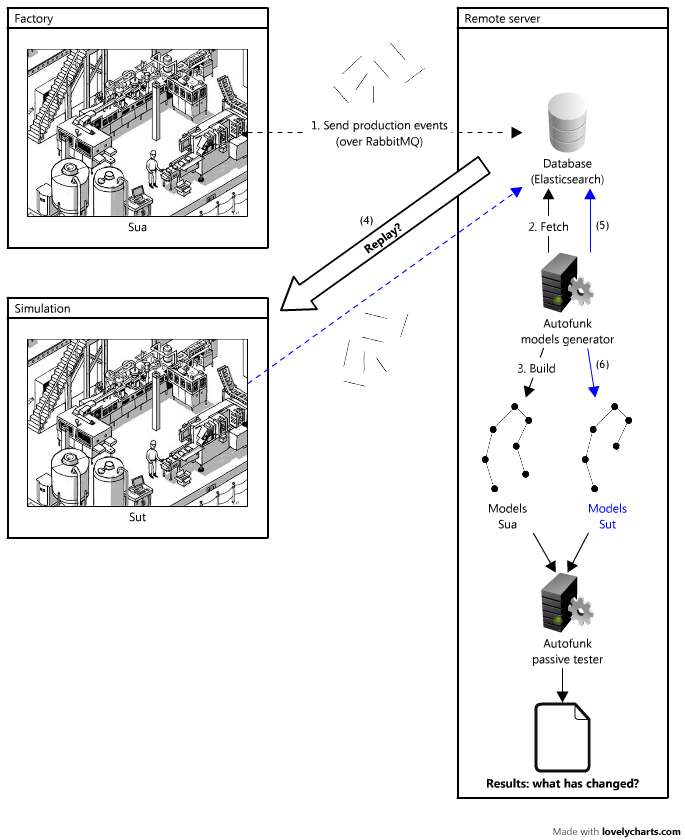
\includegraphics[width=0.96\linewidth]{figures/autofunk_active.png}
    \end{center}

    \caption{Insight of an approach discussed with Michelin to
    use a replay technique with \textit{Autofunk} in order to
    track what has changed between two versions of a production
    system.}
    \label{fig:autofunk_active}
\end{figure}
\clearpage

\subsection{Data mining}
\label{sec:conclusion:testing:data}

Data mining \cite{chakrabarti2006data} is an interdisciplinary
research domain whose goal is to extract information from a data
set. For example, visualization, which we already mentioned in a
previous section, is a component of data mining. In our case,
given the collected trace sets and/or the inferred models, we
have a lot of information available for data mining.

As an example, a side project we quickly set up with Michelin
engineers was to visualize the data collected by
\textit{Autofunk}. We relied on a tool called
\emph{Kibana}\footnote{\url{https://www.elastic.co/products/kibana}}
to show different business metrics, such as the usage rates of
some stores in a workshop, the number of manufactured products
per day, but also the usage rates of the production machines
themselves as depicted in Figure \ref{fig:kibana}. Such
information could be used to create models that might predict
maintenance operations for instance.  The main objective of
\emph{predictive maintenance} \cite{mobley2002introduction} is to
decide when to maintain a system according to its state, which we
could deduce by mining the data contained in the inferred models.

\begin{figure}[h]
    \begin{center}
        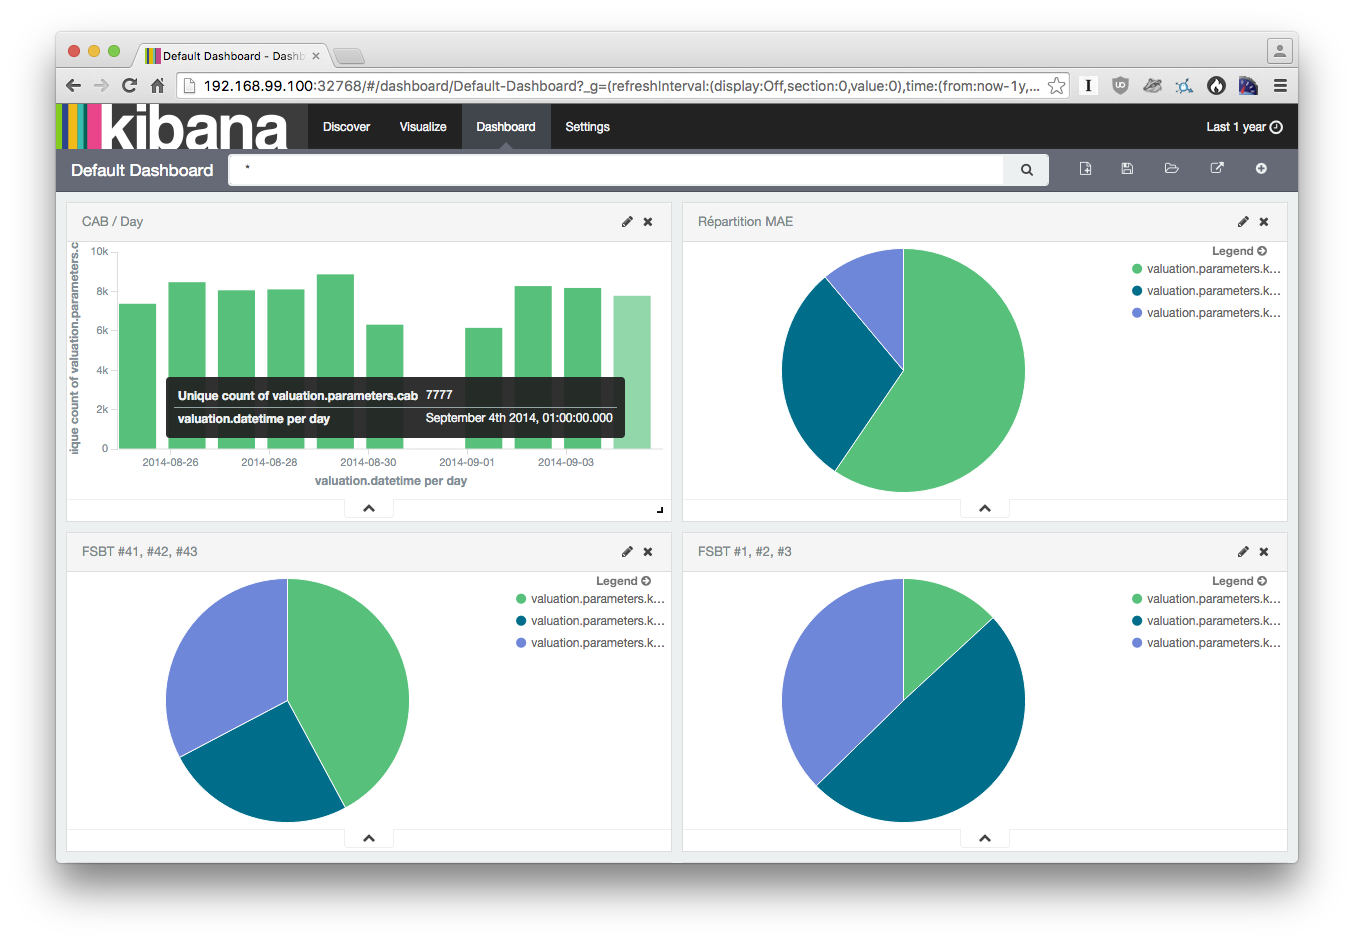
\includegraphics[width=1.0\linewidth]{figures/kibana.png}
    \end{center}

    \caption{Dashboard displaying various business metrics
    created with Kibana, a visualization tool.}
    \label{fig:kibana}
\end{figure}

We could also extract time data from the models. A potential use
case would be to detect slowness in the production lines. That
way, we might highlight imperceptible abnormal functioning
slowing down the whole manufacturing process. This is somehow
related to the \emph{workload-based performance testing} approach
introduced by Avritzer \emph{et al.} \cite{avritzer2002software},
and more generally, to the \emph{Performance Testing}
\cite{vokolos1998performance} and \emph{Knowledge Management}
\cite{pachidi2015performance} fields.

%%%%%%%%%%%%%%%%%%%%%%%%%%%%%%%%%%%%%%%%%%%%%%%%%%%%%%%%%%%%%%%%

\subsection{Refuting our main hypothesis}
\label{sec:conclusion:testing:valid}

As stated in the introduction of this thesis (cf.
\crossref{sec:intro}{sec:intro:problems}), we consider a system
under analysis as a system which behaves correctly. In other
words, such a system does not produce any fault. It is not
entirely unrealistic since this assumption has been validated
with our industrial partner Michelin. In fact, Michelin's
production systems run continuously with only a few scheduled
downtimes, \emph{i.e.} periods when either the whole factory or only a
workshop is unavailable, \emph{e.g.}, for maintenance. Otherwise systems
are fully operational.

That being said, their need for a reliable method to perform
upgrades, which led to the work presented in this thesis,
demonstrates that such systems are not error-proof. Putting it
differently, inferring models representing behaviors of a
software under analysis from production data is compelling, but
it comes at a price: it is likely that \textit{Autofunk} will
infer erroneous behaviors due to a fault that happened in a
production environment, which will not be revealed by our testing
module. It is not an issue when performing, for instance,
robustness testing, but it should not be used for conformance
testing. We were able to perform conformance testing only because
of Michelin's conditions, which we could extend to most of the
existing industrial and manufacturing contexts. Nevertheless, it
cannot be applied in all cases.

Based on this state, we would like to reject such a hypothesis to
perform conformance testing based on our inferred models, but
also to make the models more accurate. We already highlighted a
few paths to improve the accuracy of the inferred models in
Section \ref{sec:conclusion:modelinf:exact}. To go a step
further, we could apply \emph{model checking}
\cite{baier2008principles} if we consider our inferred models as
the system models. Model checking is a verification technique
that explores all possible system states, described in a
\textit{system model}, in a brute-force manner thanks to a model
checker. It is useful to show whether a given system model truly
satisfies a certain property.  Nonetheless, such properties have
to be provided, and we hit a known issue again: the lack of
up-to-date documentation and/or specification of legacy systems.
